\documentclass[../main.tex]{subfiles}

%TODO

\begin{document}

\chapter{Розробка і тестування системи}

\section{Розробка системи}

\subsection{Обґрунтування вибору засобів реалізації}

\subsection{Опис структурної (функціональної) схеми}

\subsection{Опис логічної схеми}

\subsection{Розробка бази даних}

\begin{figure}[H]
	\centering
	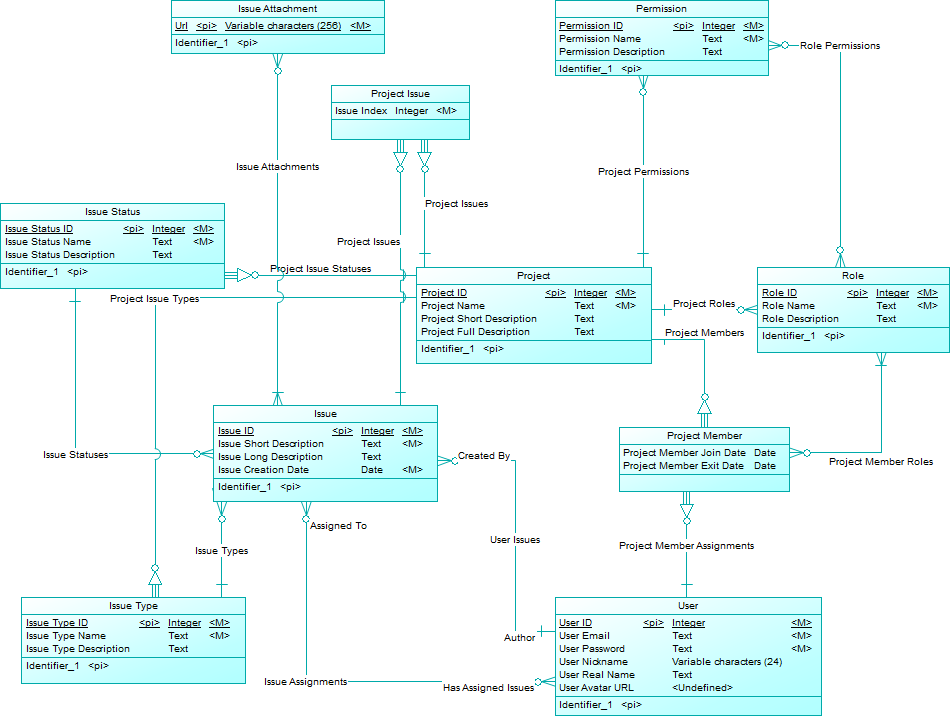
\includegraphics[width=1\textwidth]{4_db_concept}
	\caption{Концептуальна модель бази даних}
\end{figure}

\begin{figure}[H]
	\centering
	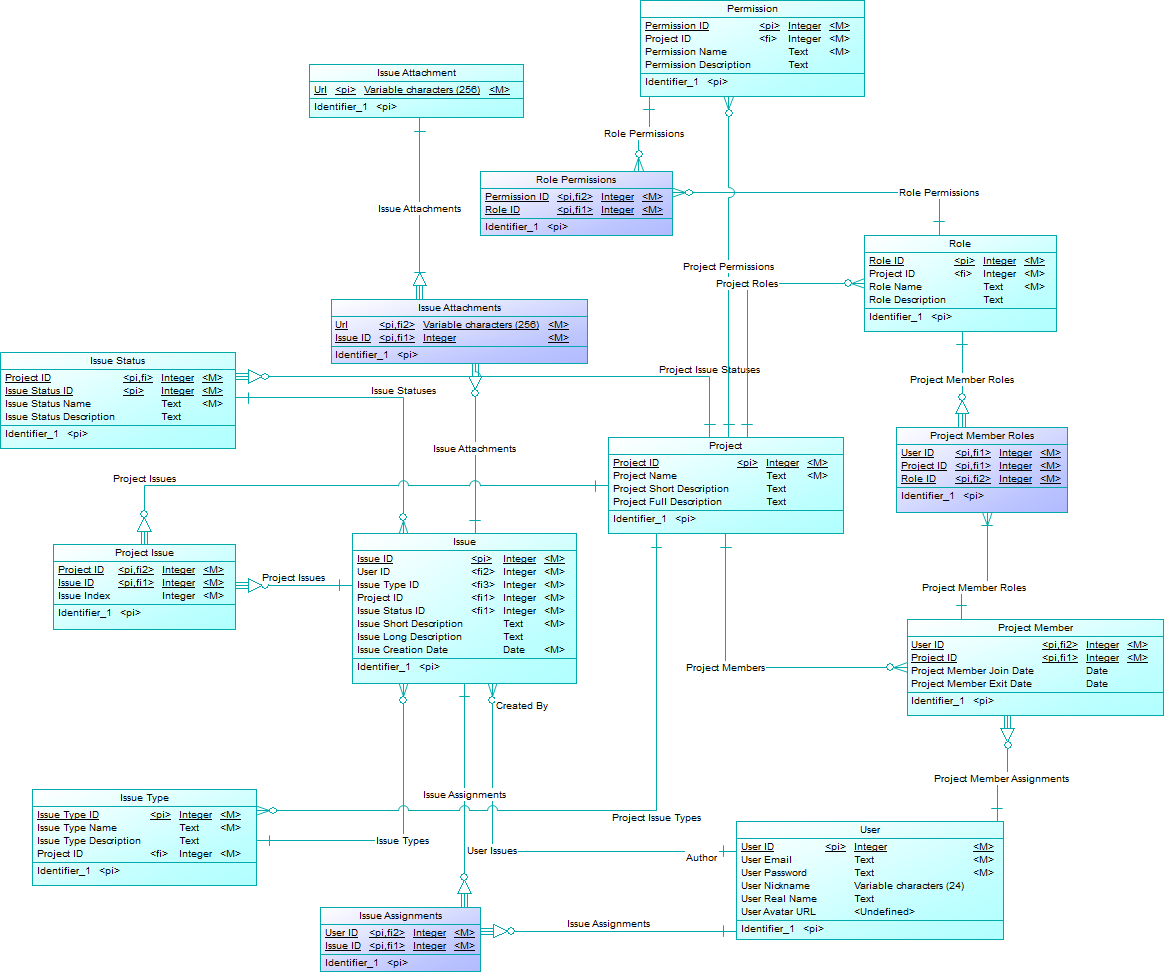
\includegraphics[width=1\textwidth]{4_db_logical}
	\caption{Логічна модель бази даних}
\end{figure}

\begin{figure}[H]
	\centering
	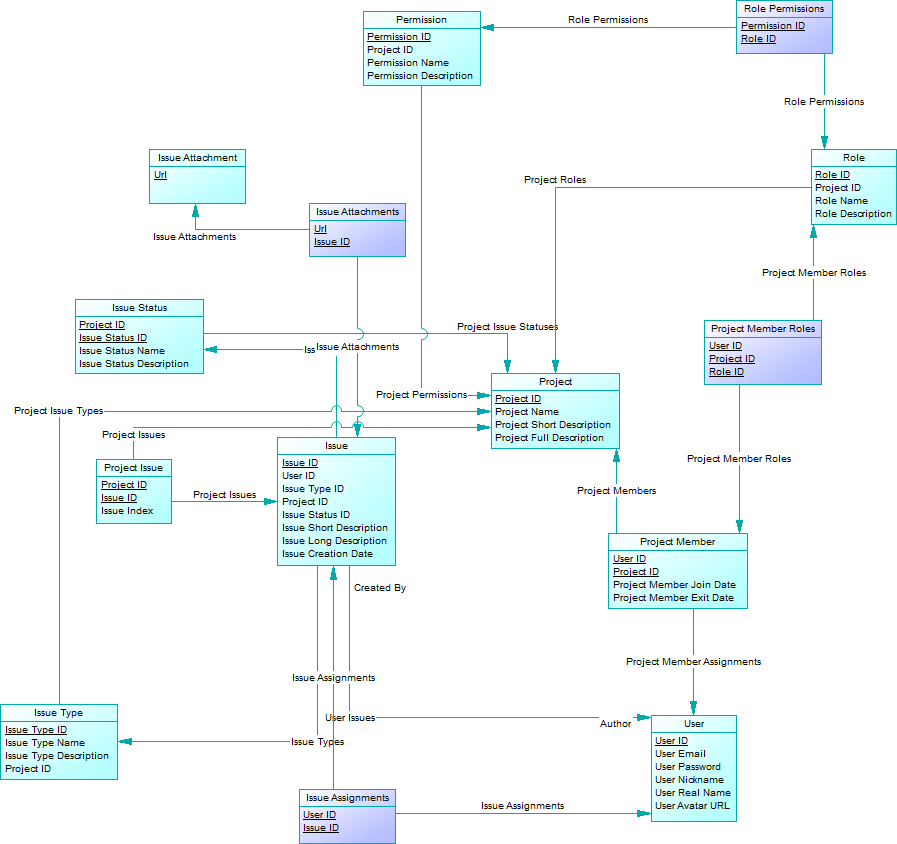
\includegraphics[width=1\textwidth]{4_db_physical}
	\caption{Фізична модель бази даних}
\end{figure}

\subsection{Розробка інтерфейсу користувача}

\subsection{Опис розробки програмних компонентів}

\chapter{Тестування інформаційної системи}

\end{document}